\chapter{Descrição do problema}\label{chapter:description}

\section{Diagrama de blocos}\label{sec:diagram}

\begin{figure}[H]
  \centering
  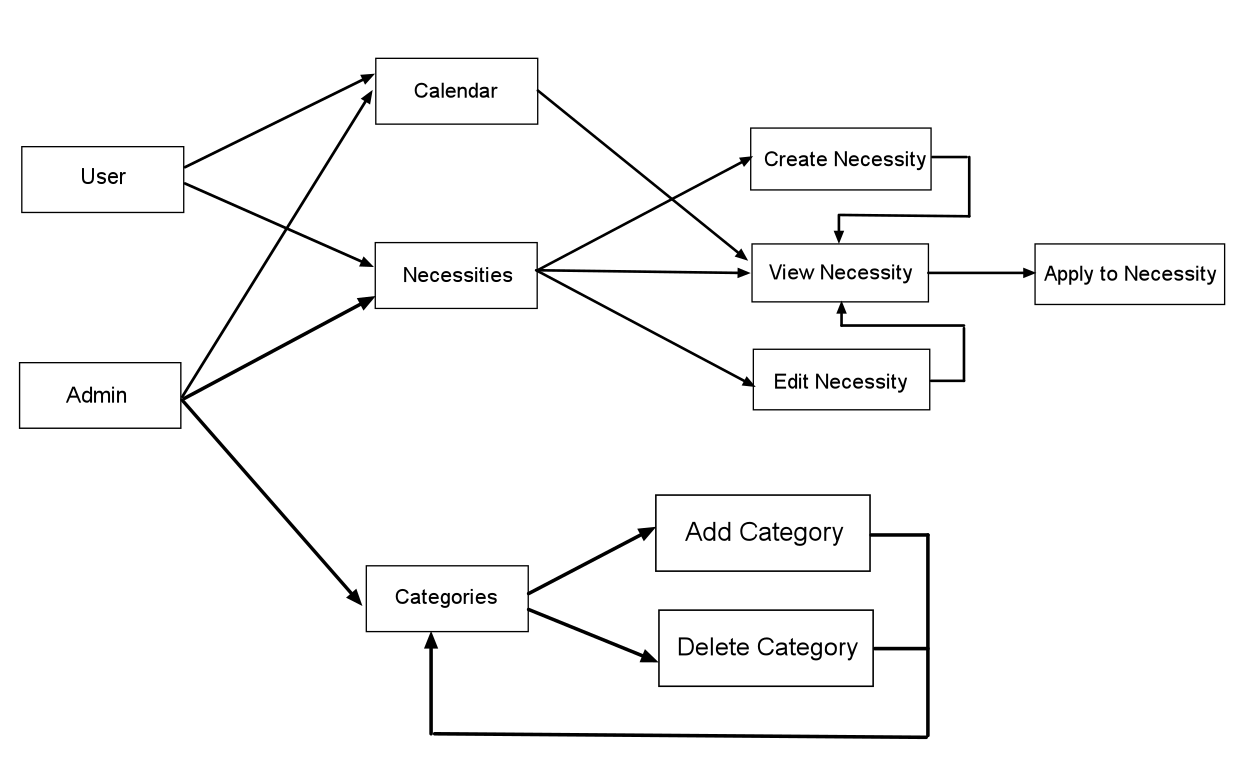
\includegraphics[scale=0.4]{figures/Diagrama de blocos.png}
  \caption{Diagrama de blocos da aplicação}\label{fig:diagram}
\end{figure}

\newpage

\section{Arquitetura}\label{sec:arquitechture}

\subsection{Plataforma \textit{OutSystems}}

A arquitetura desta plataforma pode ser observada na figura~\ref{fig:outsystemsArch}. 
O principal componente da plataforma é o Platform Server que permite que as aplicações 
desenvolvidas sejam geradas, optimizadas, compiladas e publicadas. 

\begin{figure}[H]
  \centering
  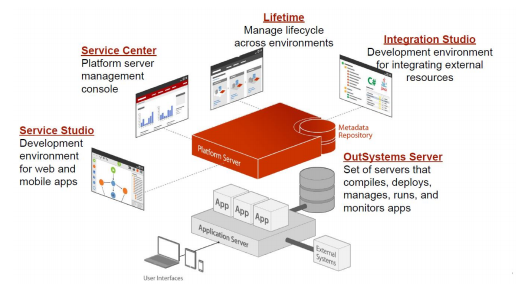
\includegraphics[]{figures/Architecture.png}
  \caption{Arquitetura da plataforma \textit{OutSystems}}\label{fig:outsystemsArch}
\end{figure}

Este componente usa os seguintes serviços: 
\begin{enumerate}
  \item \textit{Code Generator} --- Usa a aplicação modelada no \textit{Service Studio} e gera o código necessário usando tecnologias standard (como \textit{.NET, SQL Server, HTML,} etc.) para a criação de uma aplicação optimizada e segura.
  \item \textit{Deployment Services} --- Publica o código que foi previamente gerado no servidor, assegurando que a aplicação é instalada consistentemente em cada front-end da infraestrutura.
  \item \textit{Application Services} --- Gere as aplicações durante o runtime, através da execução de \textit{batches} agendados e serviços de \textit{logging} assíncronos que permitem que sejam armazenados eventos como erros, inspeções e métricas de desempenho.
\end{enumerate}

\newpage

\subsection{4 Layer Canvas}\label{sec:4lc}

Para desenharmos a arquitetura da nossa solução, seguimos a metodologia da plataforma \textit{OutSystems}, a \textit{4 Layer Canvas}.

\begin{figure}[H]
  \centering 
  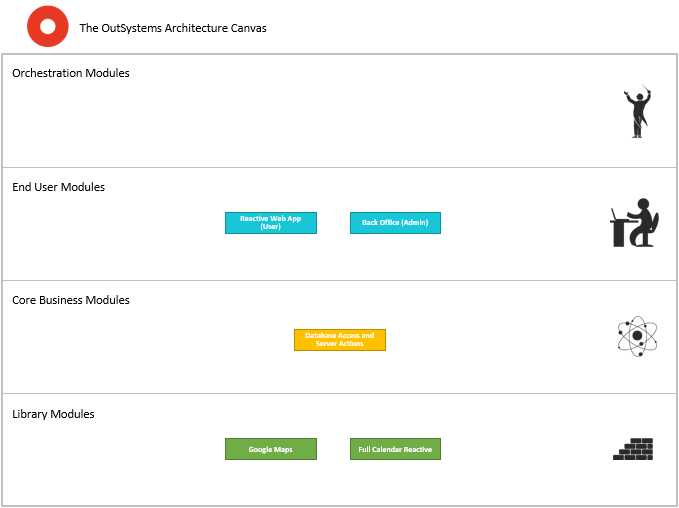
\includegraphics[scale=0.7]{figures/4LayerCanvas.png}
  \caption{4 \textit{Layer Canvas}}\label{fig:4lc}
\end{figure}

Esta metodologia propõe que se estruture as várias funcionalidades da aplicação por quatro camadas, sendo estas, começando por baixo: 

\begin{itemize}
    \item \textit{Library Layer} --- Aqui devem constar os módulos que são transversais ao domínio do problema, tais como: temas, bibliotecas, etc. 
    \item \textit{Core Layer} --- Módulos referentes à lógica de negócio, modelo de dados e \textit{server actions}. 
    \item \textit{End User Layer} --- Nesta camada é tratada toda a parte de interface e experiência do utilizador, fazendo uso das camadas anteriores. 
    \item \textit{Orchestration Layer} --- Camada que coordena a comunicação entre várias aplicações. 
\end{itemize}

É importante verificar que, apesar da metodologia apresentar quatro camadas, 
a nossa arquitetura apenas faz uso das primeiras três devido ao nosso projeto consistir em apenas uma aplicação reactive, 
e não havendo necessidade de coordenar interações com outras aplicações na camada de orquestração. 
Posto isto, a nossa aplicação assenta sobre cinco módulos, representados pela figura~\ref{fig:4lc}.

Começando pela \textit{Library Layer} verificamos que são utilizados os módulos relativos à integração da aplicação 
com o \textit{Google Maps} e com o \textit{Full Calendar Reactive}. De seguida temos a \textit{ Core Layer}, 
onde definimos as entidades de domínio e suas operações. Por fim a \textit{ End User Layer} onde são definidos 
os ecrãs e a lógica de cliente. 

\section{Modelo de Dados}\label{subsec:ModeloDados}

\begin{figure}[H]
  \centering 
  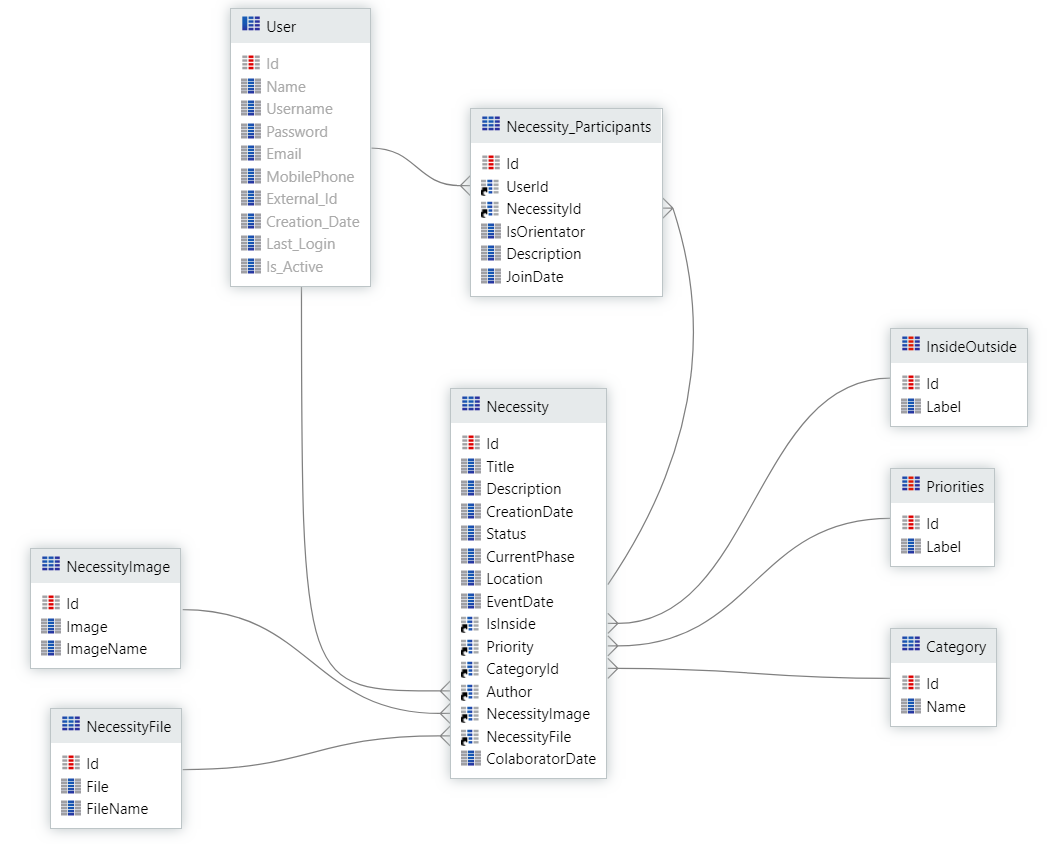
\includegraphics[scale=0.4]{figures/DataModel.png}
  \caption{Modelo de dados}\label{fig:modeloDados}
\end{figure}

O conceito predominante no modelo de dados, (figura~\ref{fig:modeloDados}), é o de necessidade, representado pela tabela \textit{Necessity}. 
Uma necessidade é caracterizada por diversos elementos dos quais destacamos o \textit{Status} que corresponde ao estado da mesma, 
podendo ter por exemplo os valores \"Arquivado\" ou \"A Decorrer\", a \textit{CurrentPhase} que indica a fase de candidaturas atual, 
podendo ser para orientadores ou participantes, e ainda a \textit{ColaboratorDate} que representa a data limite das candidaturas 
à posição de orientador. 
As tabelas \textit{NecessityImage} e \textit{NecessityFile} existem para o propósito de guardar ficheiros, 
aliviando a quantidade de dados guardada em cada tuplo \textit{Necessity}, 
seguindo também as boas práticas da plataforma \textit{OutSystems}. 
A entidade \textit{InsideOutside} serve para representar a localização das necessidades relativamente a serem 
dentro das instalações da empresa ou fora. A mesma, juntamente com a entidade \textit{Priorities} 
são entidades estáticas cuja funcionalidade é manter dados persistentes na base de dados.
Com o objetivo de guardar informação de candidaturas a necessidades, é definida a entidade \texttt{\textit{Necessities\char`_Participants}} que 
contempla o identificador da mesma, o identificador do utilizador, a descrição associada à candidatura, 
se esta candidatura é para posição de orientador ou de participante e a data da candidatura. 
Um utilizador pode ser um participante, um autor ou um orientador da necessidade. 
Este poderá ainda ter o cargo de administrador, cujos privilégios incluem editar as categorias representadas pela 
entidade \textit{Category}.

\section{Implementação}\label{sec:implementacao}

\subsection{Autenticação}\label{subsec:implementacao:login}

Para realizar a autenticação de um utilizador, este introduz as suas credenciais nos respetivos \textit{input fields} e clica no botão \textit{Login}.
Se as credenciais introduzidas não corresponderem às de nenhum utilizador na base de dados, será apresentada uma mensagem de erro.
Um utilizador só terá acesso a outros ecrãs se tiver autenticado, caso contrário será redirecionado para este ecrã.

\subsection{Dashboard}\label{subsec:implementacao:dashboard}
%LEMBRAR PARA METER AS NECESSIDADES ATIVAS NA PARTE DAS PRIORIDADES
Este é o ecrã apresentado a um utilizador autenticado assim que abre a aplicação.
O mesmo apresenta quatro \textit{widgets} que apresentam informação sobre o número de utilizadores que estão \textit{logged in} e o número de necessidades abertas com as suas respetivas prioridades (\textit{high, medium, low}).
Este ecrã apresenta também um gráfico com informação sobre as categorias existentes e a distribuição do número de necessidades criadas em cada uma das mesmas.
A seleção de uma categoria do gráfico promove a navegação para o ecrã das necessidades,  apresentando a lista das mesmas que pertencem à categoria selecionada.
Para cada uma das prioridades que as necessidades podem ter, é apresentado um \textit{ranking} dos utilizadores que mais criaram necessidades, com a respetiva prioridade.

\subsection{Visualização de necessidades}\label{subsec:implementacao:necessities}
%WHEN CSS IS DONE PUT A NICE PICTURE HERE :D
O utilizador ao carregar no botão \textit{Necessities} presente na barra da aplicação, será redirecionado para o ecrã responsável pela apresentação das necessidades. 
O intuito do mesmo consiste na apresentação das necessidades criadas pela comunidade empresarial, sendo possível aplicar filtros e/ou pesquisar pelo título de uma necessidade de modo a que sejam apresentadas apenas as necessidades alvo.
As necessidades são apresentadas num \textit{widget} tabela, cujas colunas apresentam informação relevante como título, categoria, prioridade, localização e o número de participantes até ao momento. Sempre que o utilizador pretender criar uma nova necessidade, apenas tem que carregar no botão \textit{Create Necessity} e será redirecionado para um novo ecrã, onde poderá completar a criação.
A seleção do título de uma necessidade promove a navegação para o ecrã dos detalhes da mesma. Se se verificar que o utilizador é o autor de uma das necessidades poderá editá-la carregando no ícone que aparece na ultima coluna, da linha em questão, da tabela.
A barra de pesquisa permite que o utilizador procure uma necessidade pelo seu título.
Os filtros aplicáveis são apresentados em três \textit{widgets} distintos. Dois \textit{dropdowns}, um para permitir a escolha de qual a prioridade e outro para distinguir entre necessidades no exterior e no interior das instalações da empresa.
É ainda apresentado um \textit{widget} tabela, de uma só coluna, que permite a seleção das categorias a que as necessidades pertencem, selecionando uma \textit{checkbox}.  
Sempre que exista uma mudança na seleção que algum dos \textit{widgets} de filtragem de necessidades ou uma introdução de texto na barra de pesquisa, a tabela é atualizada para apresentar apenas aquelas que verifiquem as características alvo. 

\subsection{Visualização de necessidades num calendário}\label{subsec:implementacao:calendarNecessitiesView}
%WHEN CSS IS DONE PUT A NICE PICTURE HERE :D
O utilizador ao carregar no botão \textit{Calendar} presente na barra da aplicação, será redirecionado para o ecrã responsável por mostrar, num calendário, todas as necessidades existentes organizadas por datas. 
O objetivo deste ecrã é apresentar de uma forma mais organizada e estruturada todas as necessidades criadas pela empresa, sendo possível filtrá-las. 
Para preencher o calendário, para cada necessidade, é criado um objeto \textit{Event} com a sua informação. 
Cada evento estará representado no calendário com uma cor diferente de forma a distinguir entre necessidades criadas pelo utilizador, necessidades associadas, nomeadamente uma inscrição, e necessidades criadas por outros utlizadores.
Se o utilizador carregar num evento, este é redirecionado para o seu ecrã de detalhe. 
É possível filtrar eventos pela sua categoria, através de um popover menu que contém todas as categorias existentes. 
Caso seja selecionada uma categoria, são removidos todos os eventos presentes no calendário, e de seguida, renderizado com os novos eventos filtrados.

%%%%%%%%%%%%%%%%%%%%%%%%%%%%%%%%%%%%%%%%%%%%%%%%%%%%%
\subsection{Criação e edição de necessidades}\label{subsec:implementacao:necessityCreation}
%WHEN CSS IS DONE PUT A NICE PICTURE HERE :D
O utilizador irá ser redirecionado para este ecrã sempre que tenha a intenção de criar ou alterar uma necessidade.
O ecrã apresenta os vários campos necessários para a criação ou edição da mesma.
Se o utilizador desejar editar uma necessidade, só o poderá fazer se for o autor desta.
Neste caso, o ecrã apresentará os campos já preenchidos com os dados atuais da necessidade e a possibilidade de os alterar livremente.

Os botões presentes neste ecrã são apenas dois:
\begin{enumerate}
    \item \textit{Cancel} --- apresenta um \textit{pop-up} a pedir a confirmação do utilizador, após confirmação a criação ou edição será cancelada e o utilizador redirecionado para o ecrã onde estava anteriormente.
    \item \textit{Save} --- guarda as alterações a efetuar na necessidade e cria uma ligação ao servidor para modificar a base de dados com uma nova necessidade ou alterando uma necessidade pré-existente.
\end{enumerate}